\documentclass[final,t]{beamer}
\mode<presentation>
\usetheme{c12b}
\setbeamerfont{itemize}{size=\normalsize}
\setbeamerfont{itemize/enumerate body}{size=\normalsize}
\setbeamerfont{itemize/enumerate subbody}{size=\normalsize}
\usepackage{times}
\usepackage{pifont}
\usepackage[english]{babel}
\usepackage[latin1]{inputenc}
\usepackage{todonotes}
\usepackage{listings,color}
\usepackage{graphics}
\usepackage{listings}
\usepackage[T1]{fontenc}
\usepackage{latexsym,amsfonts,url,dsfont}
\usepackage{psfrag}
\usepackage{xspace}
\usepackage{color}
\usepackage{enumerate}
\usepackage{epsfig}
\usepackage{multirow}
\usepackage{slashbox}
\usepackage{algorithm}
\usepackage[noend]{algorithmic}
\renewcommand{\algorithmiccomment}[1]{// #1}
\usepackage[orientation=portrait,size=a1]{beamerposter}

\def\Tiny{\font\Tinyfont = cmr10 at 5pt \relax  \Tinyfont}

\newcommand{\ar}{\ding{220}}
\newcommand{\diet}{\textsc{Diet}\xspace}
\newcommand{\tune}{TUNe\xspace}
\newcommand{\adage}{\textsc{Adage}\xspace}
\newcommand{\godiet}{\textsc{GoDiet}\xspace}
\newcommand{\deployware}{DeployWare\xspace}
\newcommand{\corba}{CORBA\xspace}
\newcommand{\sed}{\textsc{SeD}\xspace}
\newcommand{\seds}{\textsc{SeD}s\xspace}
\newcommand{\etc}{\emph{etc.}\xspace}
\newcommand{\ie}{\emph{i.e.,}\xspace}
\newcommand{\eg}{\emph{e.g.,}\xspace}
\newcommand{\etal}{{\em et al.}\@\xspace}
\newcommand{\gridk}{{Grid'5000}\xspace}
\newcommand{\grpc}{GridRPC\xspace}
\newcommand{\ninfg}{Ninf-G\xspace}
\newcommand{\pilgrim}{{Pilgrim}\xspace}
\newcommand{\simgrid}{{SimGrid}\xspace}

\newcommand{\fixme}[1]{\fbox{\textsl{{\bf #1}}}}
\newcommand{\fixmypar}[1]{
  \noindent
  \begin{boxedminipage}{\linewidth}
    \textsl{{\bf #1}}
  \end{boxedminipage}
}

\newcommand{\tr}[1]{\textcolor{red}{#1}}
\newcommand{\tb}[1]{\textbf{#1}}
\newcommand{\trb}[1]{\textcolor{red}{\fbox{#1}}}
\newcommand{\todoec}[2][]{\todoinline[color=gray!50,#1]{[Eddy] #2}}
\newcommand{\todomi}[2][]{\todoinline[color=yellow!50,#1]{[Matt] #2}}
\newcommand{\todoall}[2][]{\todoinline[color=red!50,#1]{#2}}
\newcommand{\todoinline}[2][]{\todo[inline,#1]{TODO: #2}}
\newcommand{\todonorm}[2][]{\todo[#1]{TODO2: #2 \xspace }}


\defbeamertemplate{bibliography item}{bigarticle}
{\lower5pt\hbox{\scalebox{2}{\pgfuseimage{beamericonarticle}}}}
% choose to show enlarged article items using that template
\setbeamertemplate{bibliography item}[bigarticle] 






\title{\hspace{0.025\linewidth}\parbox{0.10\linewidth}{
\includegraphics[width=1.\linewidth]{images/rocket.png}}\hspace{0.1\linewidth} \parbox{0.75\linewidth}{%
\Huge Energy-Aware Massively Distributed Cloud Facilities\\ the DISCOVERY Initiative}}
\author[]{\vspace{0.5cm} Fr\'ed\'eric Desprez, Shadi Ibrahim, Adrien Lebre, Anne-C\'ecile Orgerie, Jonathan Pastor and Anthony Simonet}
\institute[Discovery]{\vspace{-0.2cm}{\Large INRIA, CNRS, France - \url{http://beyondtheclouds.github.io}}\vspace{0.2cm}}
\date[Dec. 11-13, 2015]{December 11-13, 2015}
\logo{%
  \hspace{0.08\linewidth}\raisebox{-0.5\height}{
\includegraphics[width=0.15\linewidth]{images/logo_inria.pdf}}%
  \hspace{0.08\linewidth}\raisebox{-0.6\height}{
\includegraphics[width=0.075\linewidth]{images/logo_cnrs.pdf}}%
  \hspace{0.08\linewidth}\raisebox{-0.5\height}{
\includegraphics[width=0.125\linewidth]{images/rocket.png}}%
  \hspace{0.08\linewidth}\raisebox{-0.6\height}{
\includegraphics[width=0.07\linewidth]{images/Orange_logo.png}}%
  \hspace{0.08\linewidth}\raisebox{-0.6\height}{
\includegraphics[width=0.07\linewidth]{images/logo_openstack.png}}%
}


\begin{document}
\begin{frame}[fragile]{}
  \begin{columns}[t]
     \begin{column}{.49\linewidth}

      \begin{block}{\Large Centralized Cloud}
        \begin{columns}[T]
        \begin{column}{0.75\linewidth}
	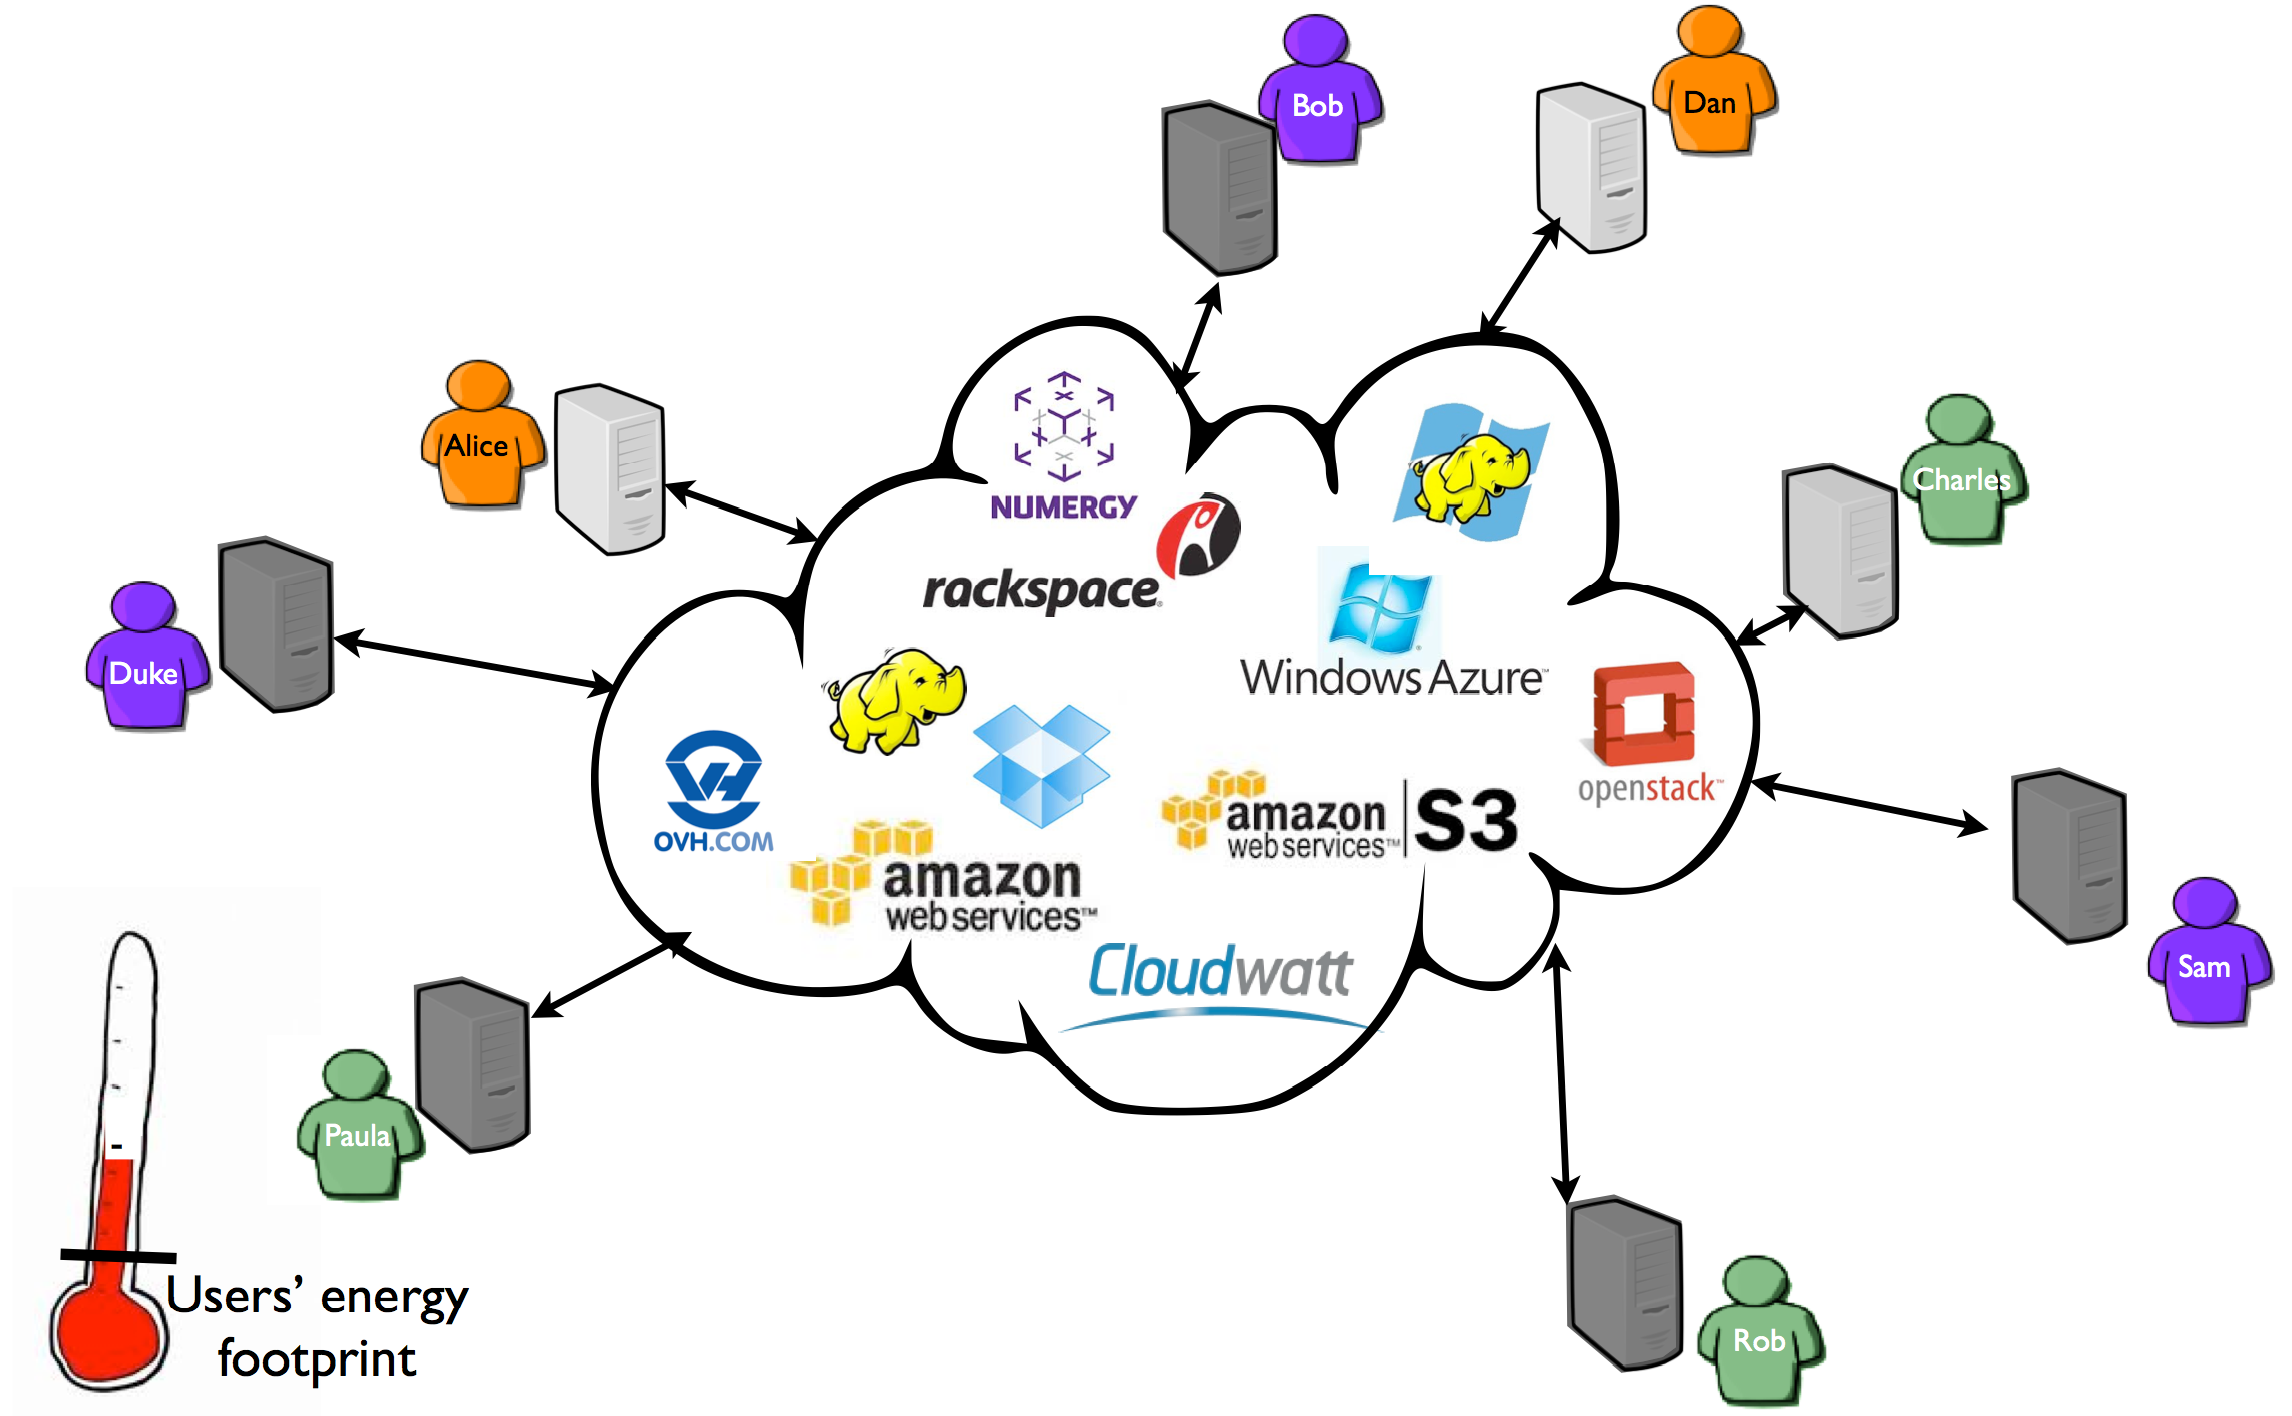
\includegraphics[width=0.9\linewidth]{images/cloud-centralise.png}
        \end{column}
        \begin{column}{0.22\linewidth}
	\textbf{\Large Drawbacks}
        \begin{itemize}
        \begin{Large}
         \item Energy consumption
         \item Scalability
         \item Reliability
         \item Locality awareness
        \end{Large}
        \end{itemize}
        \end{column}
        \end{columns}
      \end{block}


     \begin{block}{\Large OpenStack Architecture}
        \begin{columns}[T]
        \begin{column}{0.95\linewidth}
	\centering
	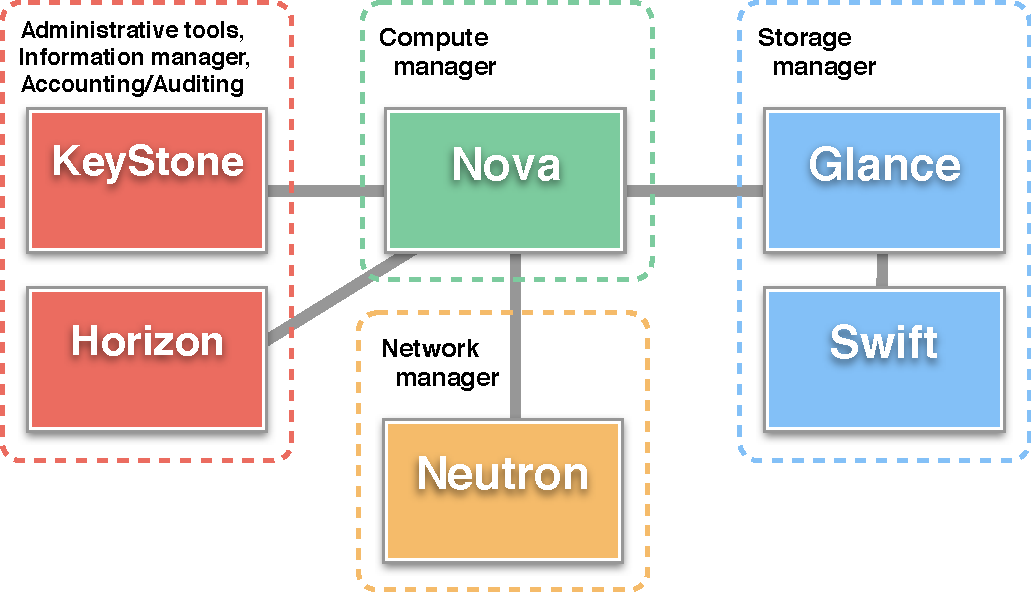
\includegraphics[width=.85\linewidth]{images/OpenStack_architecture.pdf}

        {\Large Basically OpenStack services support massive horizontal scale, but this is not the case for the entire infrastructure (database and message queue system).}
	\end{column}
        \end{columns}
      \end{block}

      \begin{block}{\Large Geant backbone network}
        \begin{columns}[T]
          \begin{column}{0.95\linewidth}
           \centering
           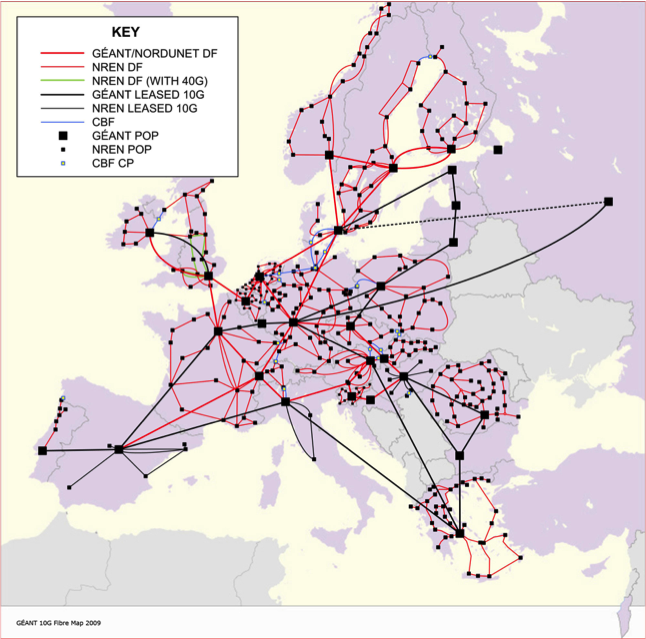
\includegraphics[width=0.95\linewidth]{images/geant.png}
          \end{column}
        \end{columns}
      \end{block}

   \end{column}


    \begin{column}{.49\linewidth}

      \begin{block}{\Large Decentralized Cloud}
        \begin{columns}[T]
        \begin{column}{0.73\linewidth}
	\begin{center}
        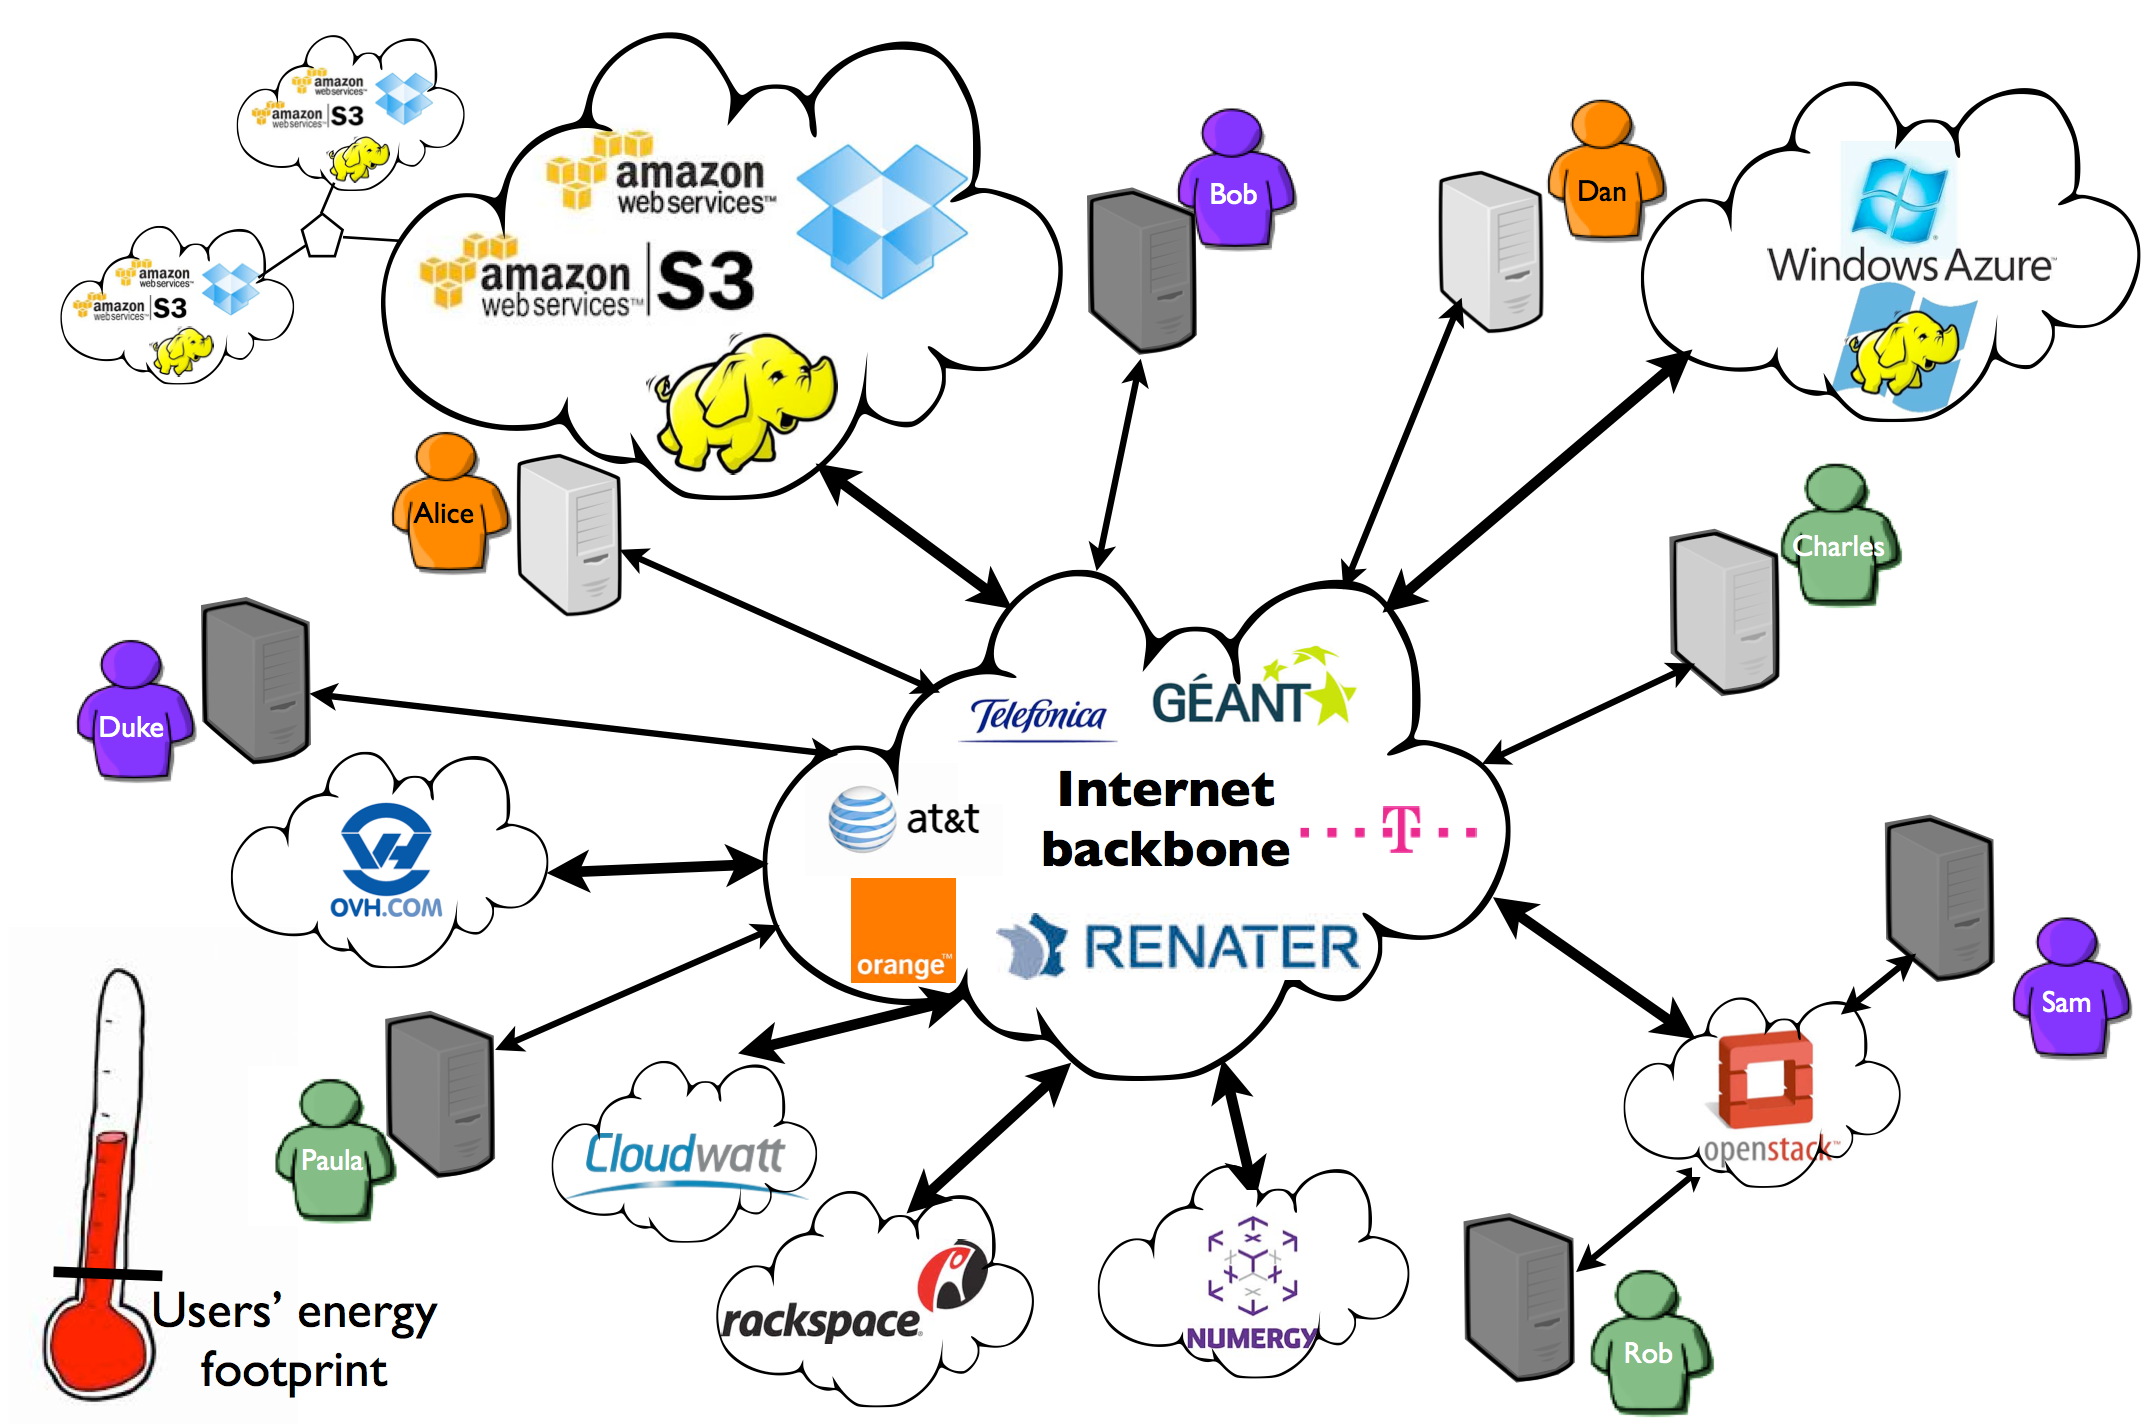
\includegraphics[width=1.\linewidth]{images/cloud-decentralise.png}
        \end{center}
        \end{column}
        \begin{column}{0.23\linewidth}
        \textbf{\Large Advantages}
        \begin{itemize}
        \begin{Large}
        \item Exploiting local renewable energy
        \item Leveraging network backbones
        \item Proposing advanced P2P overlay
        \end{Large}
        \end{itemize}
        \end{column}
        \end{columns}
      \end{block}

      \begin{block}{\Large Distributed OpenStack}
        \begin{columns}[T]

          \begin{column}{0.95\linewidth}
           \begin{flushright}
           \vspace{-4cm}
           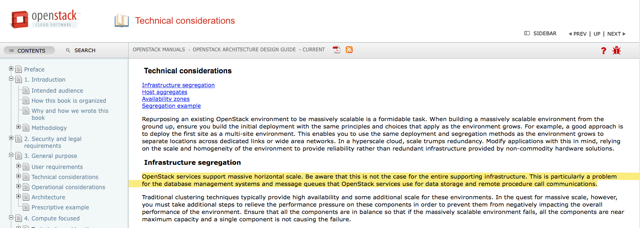
\includegraphics[width=.62\linewidth]{images/screenshot.png}
           \end{flushright}

           \centering
           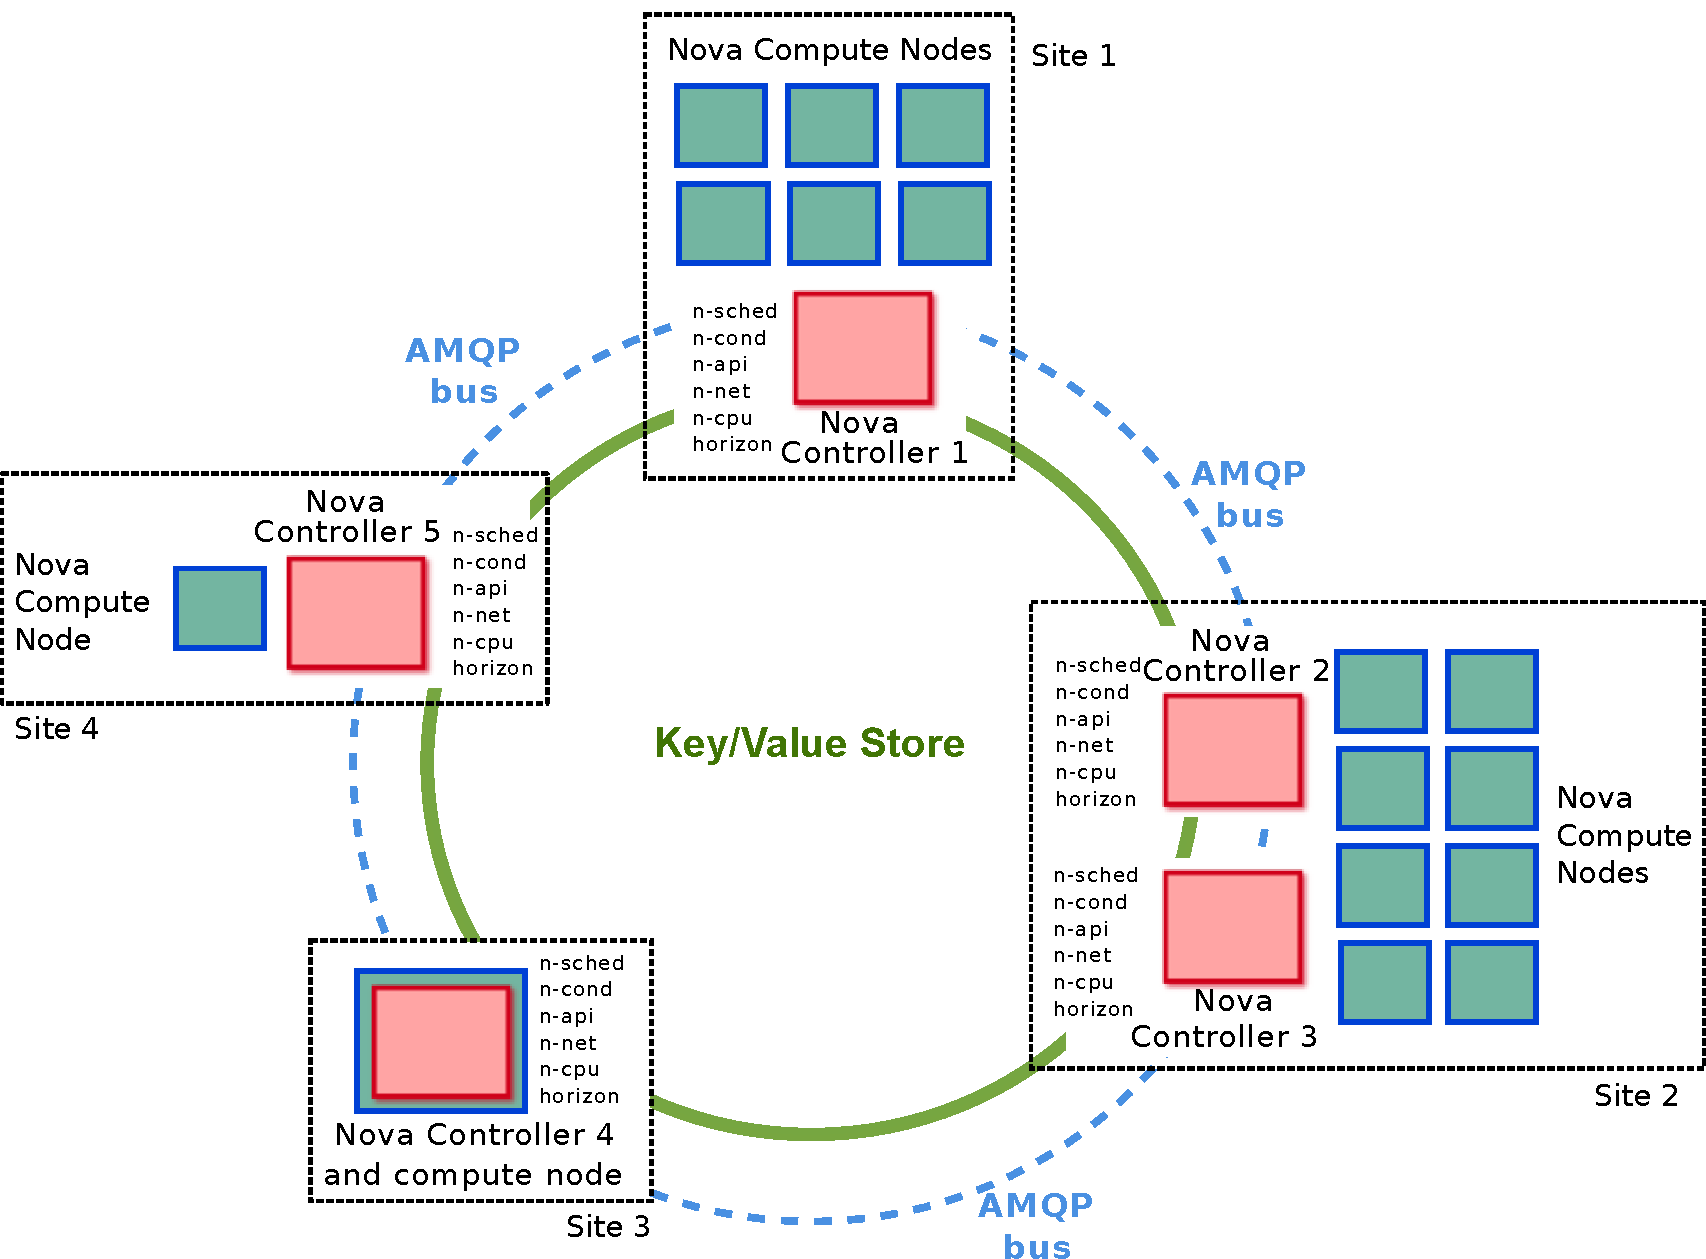
\includegraphics[width=1.\linewidth]{images/OpenStack_distributed.pdf}

          \end{column}
        \end{columns}

        \vspace{0.3cm}

        {\Large Integrating micro/nano Data Centers within the Points-of-Presence of backbone networks.}

        \vspace{0.3cm}

        {\Large Nova controllers are connected through a shared key/value backend and the AMQP bus.}
      \end{block}


      \begin{block}{\Large Energy-Awareness}
        \begin{columns}[T]
          \begin{column}{0.95\linewidth}
          \begin{itemize}
          \item {\Large Analyzing energy footprint of the OpenStack in order to identify critical components} 
          \item {\Large Performing an energy/cost-benefit analysis of a massively distributed Cloud architecture }
          \end{itemize}
          \end{column}
        \end{columns}
      \end{block}

\vspace{1cm}

\begin{block}{\Large Support}
\textit{\Large Since July 2015, the Discovery initiative is mainly supported through the Inria Project Labs program and the I/O labs, a joint lab between Inria and Orange Labs.}
\end{block}

    \end{column}

  \end{columns}








        \begin{columns}[T]
        \begin{column}{0.95\linewidth}

\vspace{0.8cm}

{\usebeamerfont*{block title} \hfill \LARGE \textcolor{i6colorscheme1}{\url{http://beyondtheclouds.github.io}} \hfill}
\vspace{0.5cm}
        \end{column}
        \end{columns}



      \begin{block}{\Large References}
        \begin{columns}[T]
        \begin{column}{0.45\linewidth}
     \vspace{-0.8cm}
      \begin{thebibliography}{1}
	\begin{normalsize}
        \bibitem{bib:ccgrid}
        {\sc A. Lebre, J. Pastor, The Discovery Consortium}
\newblock {The DISCOVERY Initiative: Overcoming Major Limitations of Traditional Server-Centric Clouds by Operating Massively Distributed IaaS Facilities}.
\newblock {\em White Paper}, 2015.
        \end{normalsize}
      \end{thebibliography}
        \end{column}

	\begin{column}{0.45\linewidth}
     \vspace{-0.8cm}
      \begin{thebibliography}{1}
        \begin{normalsize}
	\bibitem{bib:cloud}
        {\sc M. Bertier, F. Desprez, G. Fedak, A. Lebre, A.-C. Orgerie, J. Pastor, F. Quesnel, J. Rouzaud-Cornabas and C. Tedeschi}
\newblock {Beyond the Clouds: How Should Next Generation Utility Computing Infrastructures Be Designed?}.
\newblock Chapter in {\em Cloud Computing - Challenges, Limitations and R\&D Solutions}, 2014.
	\end{normalsize}
      \end{thebibliography}
        \end{column}

        \end{columns}
      \end{block}


\end{frame}
\end{document}
